\documentclass{article}
\usepackage{amsmath,amsfonts,amssymb,amscd,amsthm,pb-diagram}
\usepackage{tikz}\usetikzlibrary{fadings}
\usepackage[osf]{baskervillef}
\usepackage[affil-it]{authblk}
\def\MISS{\texttt{*** TODO ***}}
\def\fsl{\mathfrak{sl}}
\def\fso{\mathfrak{so}}
\def\fg{\mathfrak{g}}
\def\fL{\mathfrak{L}}
\def\fA{\mathfrak{A}}
\def\fM{\mathfrak{M}}
\def\fm{\mathfrak{m}}
\def\fS{\mathfrak{S}}
\def\sA{\mathcal{A}}
\def\sR{\mathcal{R}}
\def\sD{\mathcal{D}}
\def\ZZ{\mathbb{Z}}
\def\NN{\mathbb{N}}
\def\RR{\mathbb{R}}
\def\CC{\mathbb{C}}
\def\TT{\mathbb{T}}
\def\XX{\mathcal{X}}
\def\OO{\mathcal{O}}
\def\SO{\mathsf{SO}}
\def\O{\mathsf{O}}
\def\E{\mathsf{E}}
\def\fF{\mathfrak{F}}
\DeclareMathOperator{\ad}{\mathrm{ad}}
\DeclareMathOperator{\FLA}{\mathsf{FLA}}
\DeclareMathOperator{\Der}{\mathrm{Der}}
\DeclareMathOperator{\End}{\mathrm{End}}
\DeclareMathOperator{\Hom}{\mathrm{Hom}}
\DeclareMathOperator{\wt}{\mathrm{wt}}
\DeclareMathOperator{\gr}{\mathrm{gr}}
\DeclareMathOperator{\rk}{\mathrm{rk}}
\DeclareMathOperator{\pr}{\mathrm{pr}}
\DeclareMathOperator{\id}{\mathrm{id}}

\def\e{\mathsf{e}}
\def\h{\mathsf{h}}
\def\f{\mathsf{f}}

\def\p{\mathrm{p}}
\def\sm{\mathrm{sm}}
\title{Taming the infinite snake}
\author{JG}\affil{Klara Weber Institute}
\newtheorem{lem}{Lemma}
\newtheorem{prop}{Proposition}
\theoremstyle{definition}
\newtheorem{defn}{Definition}
\begin{document}
\sloppy\maketitle
\section{Introduction}
\label{sec:intro}
\subsection{Overview}
This paper is devoted to a simple mechanical
system with remarkable mathematical properties.
The \emph{infinite snake} is a sequence of 
identical rigid segments, connected by
planar rotating joints; each segment is
equipped with a wheel attached in the middle,
and the wheels roll 
on a plane with no slipping
or skidding (\textbf{figure}). The latter condition 
imposes non-holonomic constraints on the system's kinematics.
Our central claim is that
this kinematics realises, in a formal sense, the positive
subalgebra of the 
\emph{twisted loop algebra} of $\fsl_2(\RR)$. 

The statement is easy to formulate. Reducing by obvious translational
symmetry, the snake's configuration space may be identified with an
infinite torus $\TT^\infty = \varinjlim_{n\to\infty} \TT^n$, parameterising
the orientations of subsequent segments.
It is an exercise in imagination to see that the snake `follows its head':
that is, the motion of the entire system is determined by the initial configuration,
and the curve traced by the free endpoint of the first segment (\textbf{figure}). 
In particular, at every given configuration one may consider the two motions characterised
by the `head' moving along either axis of a fixed Cartesian coordinate system on the plane.
Infinitesimally, these correspond to a pair of vector fields $X$, $Y$ on $\TT^\infty$.
The Lie algebra $\fS$ generated by these two will be our main object of study.

Now, the twisted loop algebra referred to above is
$$
L_\theta\fsl_2(\RR) = \{ u(t)\ |\ u(-t)=-u(t)^T \} \subset \fsl_2(\RR)[t,t^{-1}] = L\fsl_2(\RR)
$$
where $\theta$ refers to the Cartan involution $u \mapsto -u^T$ on $\fsl_2(\RR)$.
The latter leads to a decomposition $\fsl_2(\RR) = \fso_2(\RR) \oplus \RR^2$ into eigenspaces,
and we may describe $L_\theta\fsl_2(\RR)$ as a $\ZZ$-graded Lie algebra with copies of 
$\fso_2(\RR)\simeq\RR$ in even degrees, and of $\RR^2$ in odd degrees.
The positive subalgebra $L_\theta^+\fsl_2(\RR)$ is the sum of positively graded subspaces:
$$
L_\theta^+\fsl_2(\RR) = L_\theta\fsl_2(\RR) \cap t \fsl_2(\RR)[t].
$$
Our main result then states that there is an orthogonal
basis $x,y\in\RR^2$ such that the map $X\mapsto tx$, $Y\mapsto ty$
extends to an \emph{isomorphism} of Lie algebras
$$\fS \simeq L_\theta^+\fsl_2(\RR). $$

The proof of this isomorphism is fairly non-trivial. We will exploit certain symmetries
of the snake to express the serpentine Lie algebra $\fS$ in a more abstract fashion,
and proceed with a rather explicit computation. 

\subsection{Motivaiton}
Truncating the snake's tail after finitely many segments
produces a finite system inheriting some properties of 
its infinite form. 
These finite snakes are interesting as actual
robotic systems effectuated by bending the joints (the wheels are passive). 
M. Ishikawa studied the three-segment snake in \textbf{[refs]},
coming up with a beautiful control-theoretic application of
principal connections and the Ambrose-Singer theorem. He also worked on other robots based on
effectuated joints and rigid segments with passive wheels, such as
the `trident snake' \textbf{[ref]}.

Around 2014, partly inspired by Ishikawa's work, P. Nurowski proposed 
a systematic study of the geometries associated with all snake-like systems: 
that is, planar graphs with edges corrseponding to rigid segments of fixed
length, some equipped with wheels at a fixed location along the edge. 
Given the configuration space $M$ of such a `generalised snake', 
the condition of no skidding and no skipping imposed on each wheel
gives rise to a constraint distribution $\sD \subset TM$ (one may 
exclude some degenerate configurations, thus restricting $M$ to an 
open subset over which $\sD$ has constant rank). Then one studies
the flag $\sD^\bullet$ defined inductively by $\sD^1 = \sD$,
$\sD^{i+1}=[\sD,\sD^i]$, so that $\sD^{i}$
is spanned by $i$-fold iterated Lie brackets of sections of $\sD$
(one may further shrink $M$ to an open subset over which
the $\sD^i$ have constant rank). Assuming the snake system is \emph{controllable},
i.e. that $\bigcup \sD^i=TM$, we have that $\sD^\bullet$
forms an exhaustive filtration of $TM$. One then studies the associated graded
bundle $\gr TM$, of rank equal to the dimension of $M$. By construction, the Lie
bracket of vector fields induces a Lie algebra structure in each fibre of $\gr TM$.
The graded nilpotent Lie algebra $\gr T_x M$ is called the \emph{symbol} of $\sD$ at $x$, and forms
an important local algebraic invariant of the non-holonomic distribution $\sD$.

Up to the data of segment lengths and wheel positions, these generalised snakes
are of combinatorial nature; in particular, as graphs, they admit an inductive
description, where a system is built by attaching edges (with or without wheels)
one at a time. Working in Nurowski's project, I considered the possibility of exploiting
such inductive descriptions to compute the symbol at a general configuration.
A more modest goal would be to predict the snake's \emph{growth vector}: that is
the sequence $(\rk\sD^i)_{i>0}$; equivalently, we might consider
$(\rk \gr_iTM)_{i>0}$, i.e. 
the sequence of dimensions
of graded homogeneous subspaces of the \emph{symbol} $\gr T_x M$ at a general point.
The former is the cumulative sum of the latter, which we may thus call the
\emph{growth rate vector}.

I've thus quickly arrived at the problem of computing the growth vector of
the $n$-segment snake -- the result of iteratively attaching a wheeled edge  
to a free endpoint of the system. An explicit calculation with help of computer
algebra gives the following results:
\begin{center}\fbox{
\begin{tabular}{c|l||c|l||c|l}
        $n$ & growth rate&
        $n$ & growth rate&
        $n$ & growth rate\\
        \hline
        1 & 2 1 & 
        4 & 2 1 2 1 &
        7 & 2 1 2 1 2 1
        \\
        2 & 2 1 1 &
        5 & 2 1 2 1 1 &
        8 & 2 1 2 1 2 1 1 
        \\
        3 & 2 1 2 &
        6 & 2 1 2 1 2 &
        9 & 2 1 2 1 2 1 2
\end{tabular}
}\end{center}
A clear pattern emerges -- how does one explain it?
Up to some irregularity at the `tail', the growth rate
vector appears to be a string of 2 1 2 1 2 1 2 \dots,
suggesting that the results for finite snakes may be the shadow
of a simpler situation in the limit $n\to\infty$. 

There are some remarkable features of the snake to be pointed out in this context.
First, the symbol (at a general point) of each of the $n$-segment
snakes appears to have \emph{width} 2 (that is the bound on
the dimensions of homogeneous graded components). This is
very far from the generic situation, and puts the sequence
of snakes in a similar category as the much studied sequence
of \emph{trailers}, systems with growth rate 2 1 1 1 \dots (indeed, deforming the $n$-segment snake
by varying the position of the wheels, and then degerating by moving each wheel to
an endpoint of its segment, one ends up with an $n$-segment trailer). 
Second, in the infinite snake, the symbol of $\sD$ actually coincides with
the Lie algebra generated by the vector fields $X, Y$ spanning $\sD$ (that doesn't
happen for finite snakes, where -- unlike the symbol -- the algebra generated
by the two vector fields isn't nilpotent).
All these points will be taken up more formally in Section \ref{sec:further}.

\subsection{Approach}
It is easy to \emph{conjecture} the isomorphism $\fS \simeq L^+_\theta\fsl_2(\RR)$
based on explicit computation,\footnote{I've presented the conjecture and some of its
ramifications at a 2015 Bedlewo workshop on Nonlinear Control.}
but actually proving it requires tackling two infinities: the depth of iterated Lie brackets,
and the length of the snake.
The former involves straightforward induction on bracket depth.
The latter will be approached through a less obvious \emph{corecursion}.

The corecursion is related
to a particular `symmetry' of the infinite snake that becomes broken
in its finite sub-snakes:
namely, the tail, that is the
snake minus its initial segment,
is still an infinite snake.\footnote{Of course cutting the snake's head off
is not invertible, whence one should rather speak of a \emph{pseudo-}symmetry.}
This gives rise to a `shift operation', passing from the original snake to its
tail. We shall furhter twist it using the obvious Euclidean symmetry of the system
(since we have already reduced the configuration space by translations,
we are left with rotations and reflections). 

So far, we haven't really specified the parameterisation identifying the infinite snake's
reduced configuration space with $\TT^\infty$. Let us temporarily denote the
former more abstractly as $M$. Now, identify the configuration space
of the one-segment snake with $\TT$, parameterised by an angle coordinate $\varphi$
such that $\varphi=0$ corresponds to the segment being aligned with the first
Cartesian axis (the one associated with $X$). Let $$ \TT \xleftarrow{\pi_h} M \xrightarrow{\pi_t} M $$
be the projections sending the configuration $m$ of an infinite snake 
to, respectively, the configuration of its initial segment, $\pi_h(m)$,
and the configuration
of its tail \emph{as} an infinite snake, $\pi_t(m)$.
Now, let $$ S, R_\vartheta : M \to M $$
denote the symmetries induced by, respectively,
reflection about the first Cartesian axis, and
rotation by $\vartheta \in \TT$. Define
$$ R : \TT \times M \to M,\quad R(\vartheta, m) = R_\vartheta(m) $$ 
and 
consider the \emph{invertible} map
$$
\Phi : M \xrightarrow{\langle \pi_h,\pi_t\rangle} \TT \times M
\xrightarrow{\langle \pr_1, S \circ R\rangle} \TT \times M.
$$
That is, $\Phi$ sends a configuration of the infinite snake
to the pair: the configuration of its initial segment, and
the configuration of its tail, but in a coordinate system
whose first axis is parallel to the initial segment, and
whose orientation is reflected.

Iterating the map $\Phi$ produces a sequence of invertible maps
$\Phi^{(n)} : M \to \TT^n \times M$ and, in the limit,
an identification 
$$\pr_1 \circ \Phi^{(\infty)} : M \longrightarrow \TT^\infty = \varprojlim_{n\to\infty} \TT^n.$$
With standard angle coordinates $(\varphi_1,\varphi_2,\dots)$ on $\TT^\infty$,
the above identification corresponds to parameterising the infinite snake
as in Figure~\ref{fig:param}.

\begin{figure}\begin{center} % snake, parameterisation
        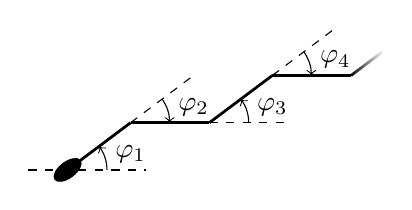
\begin{tikzpicture}
                \draw[dashed] (-0.5,0) -- (1.0,0);
                \draw[line width=1] (0,0) -- (0.8,0.6);
                \draw[dashed] (0.8,0.6) -- (1.6,1.2); 
                \draw[line width=1] (0.8,0.6) -- (1.8,0.6); 
                \draw[dashed] (1.8,0.6) -- (2.8,0.6);
                \draw[line width=1] (1.8,0.6) -- (2.6,1.2); 
                \draw[dashed] (2.6,1.2) -- (3.4,1.8); 
                \draw[line width=1] (2.6,1.2) -- (3.6,1.2); 
                \draw[line width=1,path fading=east] (3.6,1.2) -- (4.0,1.5);
                \draw[->] (0.5,0) arc (0:36:0.5); \node at (0.8,0.2) { $\varphi_1$ };
                \draw[->] (2.3,0.6) arc (0:36:0.5); \node at (2.6,0.8) { $\varphi_3$ };
                \draw[->] (1.2,0.9) arc (36:0:0.5); \node at (1.6,0.8) { $\varphi_2$ };
                \draw[->] (3.0,1.5) arc (36:0:0.5); \node at (3.4,1.4) { $\varphi_4$ };
                \draw[rotate=37,fill] (0,0) ellipse (0.2 and 0.1);        
        \end{tikzpicture}\end{center}
        \caption{Parameterisation defined by $\pr_1\circ\Phi^{\infty} : M \to \TT^\infty$.
        \label{fig:param}}
\end{figure}

It turns out that the vector fields $X$, $Y$ admit a convenient corecursive
description with respect to $\Phi$. Let $\XX^\p(M)$ denote the space of
smooth projectable vector fields on $M$ (that is an inverse limit of 
spaces of smooth projectable vector fields on the configuration spaces of finite sub-snakes),
and let
$$ \XX(\TT) \xrightarrow{\iota} \XX^\p(M) \xleftarrow{\Sigma} \XX^\p(M) $$
be the maps induced by $\Phi^{-1} :  \TT\times M \to M$. Note that these in turn induce
an isomorphism\footnote{For simplicity, at this stage we use
smooth functions, whence the need for a completed tensor product.
In Sec.~\ref{sec:algebra} we will actually 
work with Laurent polynomials on complex tori.}
$$
\XX(\TT) \oplus C^\infty(\TT) \widehat\otimes \XX^p(M) \to \XX^\p(M),
\quad
(v, f \otimes V) \mapsto \iota v + (\pi_h^* f)\cdot \Sigma V.
$$
It will be most convenient to complexify and consider
$Z = X+iY \in \CC\otimes\XX^\p(M)$.
Then, we find the following corecursive formula (see Section~\ref{sec:basic}):
$$
Z = -e^{i\varphi} \left( 
        \Sigma Z + i(\Sigma-1)\iota\partial_\varphi
\right)$$
where we view $\varphi$ as a function on $M$ via $\pi_h^*$.
Since the operator $1+e^{i\varphi}\Sigma$ 
is invertible on $\XX^\p(M)$, the above does indeed determine $Z$. A
conjugate formula holds for $\overline Z = X - iY$, and it is not unreasonable
to expect such recursive formulas for their iterated Lie brackets.
These are derived in Section \ref{sec:algebra}. In particular,
we find that the Lie algebra $\fS_\CC$ generated by $Z, \overline Z$
(a complexification of $\fS$) is isomorphic to $L_\theta^+\fsl_2(\CC)$.
Then, passing to real forms we conclude with $\fS\simeq L_\theta^+\fsl_2(\RR)$.


\subsection{Consequences}

\subsection{Acknowledgements}


\section{Basic construction}
\label{sec:basic}
\subsection{A single segment}
Given the inductive construction of the snake system,
it is clear we need to begin with studying the behaviour of a single
segment. We are interested with how the single segment's kinematics
translate the motions of one endpoint into those of the other -- for then,
viewing the infinite snake as a chain of segments, we will be able
to propagate the motions of its head toward subsequent joints, along the tail. 
Remarkably, the Lie algebra $\fsl_2(\RR)$ shows up already at this stage. 
What
we state here is not new, and may be pursued far deeper (cf. {\bf[BorLeviPerlineTabachnikov:TireTracks]}).
\emph{The notation used hereafter will at times differ from that of the previous section.}


\begin{figure} % one segment; transfer
        \begin{center}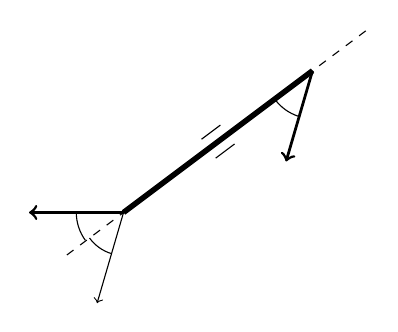
\begin{tikzpicture}[scale=0.6]
                \draw[line width=2] (0,0) -- (4,3);
                \draw[dashed] (-1.2,-0.9) -- (5.2,3.9);
                \draw (1.95,1.15) -- (2.35,1.45);
                \draw (1.65,1.55) -- (2.05,1.85);
                \draw[->, line width=1] (0,0) -- (-2,0);
                \draw[->] (0,0) -- (-0.56,-1.92);
                \draw[->,line width=1] (4,3) -- (3.44,1.08);
                \draw (-1,0) arc (180:216:1);
                \draw (3.2,2.4) arc (216:252:1);
                \draw (-0.72,-0.54) arc (216:252:0.9);
        \end{tikzpicture}\end{center}
        \caption{End-to-end translation in a single segment (all indicated angles
        are equal).\label{fig:seg}}
\end{figure}

Let $M_1$ be the configuration space of the single segment, moving along
a Euclidean plane identified with $\RR^2$.
Assume the segment has unit length, and fix an ordering of its two endpoints.
We then have three well-defined projections:
$$
 \varphi : M_1 \to \TT,\quad p_0, p_1 : M_1 \rightrightarrows \RR^2
$$
mapping the segment's configuration to, respectively,
its orientation, and the positions of the two endpoints.
Both $\langle p_i,\varphi\rangle : M_1 \to \RR^2\times\TT$
are diffeomorphisms.
Identifying $\TT$ with the unit circle in $\RR^2$, we have the relation
\begin{equation}\label{eq:seg-rel} p_1(m) - p_0(m) = \varphi(m)\quad\textrm{for}\ m \in M_1.\end{equation}
Identifying $T_{p_0(m)}\RR^2, T_{p_1(m)}\RR^2$ with $\RR^2$
using the Euclidean structure,
the no-slip-or-skid condition
on $v \in T_m M_1$ becomes 
\begin{equation}
        \label{eq:seg-cons}
        (p_{0*}v + p_{1*}v) \wedge \varphi(m) = 0\quad \textrm{in}\ \Lambda^2\RR^2.
\end{equation}
Let us further identify $T_{\varphi(m)}\TT \simeq \RR$  and $\Lambda^2\RR^2 \simeq \RR$
using the Euclidean structure on $\RR^2$.
\begin{lem}\label{lem:seg-trans}
        Suppose $v \in T_m M_1$ satisfies \eqref{eq:seg-cons}. Then
        \begin{align}
                p_{1*}v & = S_{\varphi(m)}\  p_{0*}v,\\
                \varphi_*v&= -2\varphi(m)\wedge p_{0*}v,
        \end{align}
        where $S_u \in \End\RR^2$ denotes reflection in the axis $\RR u$ for $u \in \TT$.
\end{lem}
\begin{proof}
        Let $P_u \in \End\RR^2$ be the orthogonal projection onto $\RR u$ for $u \in \TT$.
        By \eqref{eq:seg-cons}, $(1-P_{\varphi(m)}) p_{1*}v = - (1-P_{\varphi(m)}) p_{0*}v$. On the other hand,
        differentiating \eqref{eq:seg-rel} we have $P_{\varphi(m)} p_{1*}v=P_{\varphi(m)} p_{0*}v$. It follows that
        $p_{1*}v = (2P_{\varphi(m)}-1)p_{0*v} = S_{\varphi(m)}p_{0*v}$, proving the first formula.
        Using \eqref{eq:seg-rel} again 
        we have $$\varphi_* v = p_{1*}v-p_{0*}v = (S_{\varphi(m)}-1) (p_{0*}v) = -2(1-P_{\varphi(m)}) (p_{0*}v)$$
        in $\RR^2$.
        Since $(u\wedge) \circ (1-P_u) = (u\wedge)$ for $u \in \TT$, the second formula follows
        once one identifies $T_{\varphi(m)}\TT\simeq\RR\simeq\Lambda^2\RR^2$.
\end{proof}
In other words, the infinitesimal motions of the two endpoints
are related by a reflection in the axis spanned by the segment,
see Figure~\ref{fig:seg}. As a consequence, movement of the first endpoint 
determines that of the second endpoint, a property we will use to
propagate motion along the actual snake. 
It also determines the evolution of the orientation of the segment.
\begin{lem}\label{lem:seg-iso}
Let $\sD_1 \subset TM_1$
denote the subset consisting of vectors $v$ satisfying
\eqref{eq:seg-cons}. Then $\sD_1$ is a rank $2$ vector
sub-bundle, and each of $$p_{i*}|_{\sD_1} : \sD_1 \to p_i^* T\RR^2 \simeq
M_1\times\RR^2$$ is a vector bundle isomorphism.
\end{lem}
\begin{proof}
        Using the diffeomorphism $\langle p_i,\varphi\rangle : M_1 \to \RR^2\times\TT$,
        the claim follows from Lemma \ref{lem:seg-trans}.
\end{proof}

The Euclidean group $\E_2 \simeq \RR^2 \rtimes \O_2(\RR)$ of $\RR^2$ 
acts on $M_1$ so that $p_0,p_1$ are equivariant. 
Letting the translation subgroup $\RR^2$ act trivially on $\TT$,
and the factor $\O_2(\RR)$ naturally (via $\TT \subset \RR^2$),
we have that
$\varphi : M_1 \to \TT$ is equivariant as well,
and identifies $\TT$ with the quotient $M_1/\RR^2$.
The distribution $\sD_1 \subset TM_1$ is preserved by $\E_2$, and in particular
by $\RR^2$.
We may thus consider the map
\begin{equation}
        \label{eq:xi1}
        \xi_1 : \RR^2 \xrightarrow{ p_{0*}^{-1}}  \Gamma(M_1,\sD_1)^{\RR^2} \xrightarrow{\varphi_*} \XX(\TT) 
\end{equation}
where $\Gamma(M_1,\sD_1)^{\RR^2}$ is the space of translation-invariant sections of $\sD_1$.
Given a vector $v \in \RR^2$, dragging the first endpoint
of the segment along $v$ produces $\xi_1(v)$ as the corresponding
vector field on the \emph{reduced} configuration space $\TT$ of the segment.
Remarkably, these vector fields generate the `standard' infinitesimal action of $\fsl_2(\RR)$
on the circle.
\begin{lem}\label{lem:seg-sl2}
        Let $\fsl_2(\RR) = \fso_2(\RR) \oplus \fm$ be the decomposition
        of the Lie algebra $\fsl_2(\RR)$ into eigenspaces of the Cartan
        involution $x\mapsto-x^T$. Then there exists a Lie algebra monomorphism
        $$ \eta : \fsl_2(\RR) \to \XX(\TT) $$
        and an $\SO_2(\RR)$-equivariant isomorphism $\fm\simeq\RR^2$
        such that:
        \begin{enumerate}
                \item $\eta|_{\fso_2(\RR)}$ acts naturally by infinitesimal rotations of $\TT\subset \RR^2$,
                \item $\eta|_\fm$ coincides with $\xi_1$ under $\fm\simeq\RR^2$.
        \end{enumerate}
        Furthermore, up to $\SO_2(\RR)$-conjugacy, $\eta$ is determined by condition (1) alone.
\end{lem}
\begin{proof}
        Let us compute explicitly with a standard Euclidean basis $e_1,e_2 \in \RR^2$
        and an angle coordinate $\phi$ on $\TT$. Let $r \in \fso_2(\RR)$ be a generator
        acting as $\eta(r)=\partial_\phi$ (thus satisfying condition (1) of the Lemma), 
        and $p,q \in \fm$ a basis such that
        $[r,p]=-q$, $[r,q]=p$, $[p,q]=r$.
        Then, writing $\eta(p) = f_p(\phi)\partial_\phi$ and $\eta(q) = f_q(\phi)\partial_\phi$ and
        imposing the above Lie brackets,
        one finds 
        $$ \eta(p) = \cos(\phi-\phi_0)\ \partial_\phi,\quad \eta(q) = \sin(\phi-\phi_0)\partial_\phi $$
        for some $\phi_0$. Choosing $\phi_0=-\pi/2$ makes the isomorphism
        $$ \RR^2 \to \fm,\quad e_1 \mapsto p,\quad e_2\mapsto q $$
        satisfy condition (2).
\end{proof}

\subsection{Growing the tail}

An $n$-segment snake is a sequence of individual segments, chained at their endpoints.
We may thus define its configuration space as 
$$ M_n = M_1 \times_{\RR^2} \cdots \times_{\RR^2} M_1\quad\textrm{($n$ factors)} $$
where we use $p_1 : M_1 \to \RR^2$ for the left-hand factor
and $p_0 : M_1 \to \RR^2$ for the right-hand factor as
structure maps in each fibre product
$-\times_{\RR^2}-$.
Using $s_k : M_n \to M_1$ for a projection onto the $k$-th factor, $1\le k\le n$,
we have $p_1s_k = p_0s_{k+1}$ with $k<n$. Let us set
$$ p^n_0 = p_0s_1,\quad p^n_k = p_1s_k\ \textrm{for}\ 1\le k\le n. $$
Now, a trajectory of the $n$-segment snake, i.e. a curve in $M_n$, satisfies
the constraints if its projection under each $s_k$ satisfies the constraints
as a one-segment trajectory. The constraint distribution of the $n$-segment snake
is thus given by:
$$
TM_n\supset \sD_n = \bigcap_{k=1}^n s_k^{-1} \sD_1.
$$
\begin{lem}\label{lem:n-iso}
$\sD_n \subset TM_n$ is a rank $2$ sub-bundle, and
$s_{k*}:\sD_n \to s_k^*\sD_1$ is an isomorphism for each $1\le k\le n$.
\end{lem}
\begin{proof}
        By construction, $\sD_n$ is (canoncally isomorphic to) the limit of the diagram
        $$\begin{diagram}
                \node{} \node{s_1^*\sD_1}\arrow{sw,t}{s_1^* p_{0*}}\arrow{se,t}{s_1^* p_{1*}}
                \node{} \node{s_2^*\sD_1}\arrow{sw,b}{s_2^* p_{0*}}\arrow{se}
                \node{} \node{\cdots}\arrow{sw}\arrow{se}\\
                \node{p^{n*}_0 T\RR^2} \node{} \node{p^{n*}_1 T\RR^2}
                \node{} \node{p^{n*}_2 T\RR^2}\node{}\node{p^{n*}_n T\RR^2.}
        \end{diagram}
        $$
        By Lemma \ref{lem:seg-iso}, 
        the maps $\sD_1 \to p_i^* T\RR^2$, $i=0,1$, are isomorphisms,
        and thus so are the maps in the above diagram.
        It then follows that the canonical projections $\sD_n \to s_1^*\sD_k$, $1\le k\le n$
        from the limit are themselves isomorphisms.
\end{proof}
Given a somewhat abstract proof, let us note that the interpretation is simple:
the motion of the entire $n$-segment snake is determined by that of any of its segments.
Further, by Lemma \ref{lem:seg-iso}, it is in fact determined by the motion of the head
or any of the joints. In particular thus,
$$ p_{0*}^n : \sD_n \to p_0^{n*}T\RR^2 \simeq M_n \times \RR^2 $$
is an isomorphism.
The translation action of $\RR^2$ on each factor $M_1$ induces an action
on $M_n$, preserving $\sD_n$ and 
making each $p^n_k$ equivariant.
We may, analogously to \eqref{eq:xi1}, consider the map
$$
\xi_n : \RR^2 \xrightarrow{(p_{0*}^n)^{-1}} \Gamma(M_n, \sD_n)^{\RR^2} \to
 \XX(M_n/\RR^2)
$$
into vector fields on the \emph{reduced configuration space} $M_n/\RR^2$.

Note that $\langle \varphi s_1,\dots,\varphi s_k\rangle : M_n \to \TT^n$ 
is an $\RR^2$-principal bundle (for the translation action), thus providing
a diffeomorphism
$M_n/\RR^2 \simeq \TT^n$. We don't want to identify the two at this stage,
so we'll write $\overline M_n = M_n/\RR^2$, equipped with the map
$$\xi_n:\RR^2 \to \XX(\overline M_n).$$ Now, for $m<n$, projection $M_n\to M_m$ onto 
the first $m$ factors induces a map
$$ \pi^n_m : \overline M_n \to \overline M_m. $$
We will say that a vector field $\upsilon \in \XX(\overline M_n)$ is \emph{projectable},
if $\pi^n_{m*}\upsilon \in \XX(\overline M_m)$ is well-defined for all $1 < m < n$.
The space of projectable vector fields on $\overline M_n$ is closed under the Lie bracket,
and we denote it $\XX^\p(\overline M_n)$.

\begin{lem}\label{lem:xi-proj}
        $\xi_n$ is projectable, and $\pi^n_{m*}\circ\xi_n = \xi_m$ for $0 < m < n$.
\end{lem}
\begin{proof}
        $p^n_{0*} = p^m_{0*} \circ \pi^n_{m*}$ as maps $\sD_n \to T\RR^2$.
\end{proof}


The $\pi^n_m$, $0 < m < n$ form a \emph{projective system},
and we would like to consider its (infinite-dimensional) limit $$\overline M_\infty = \varprojlim \overline M_n $$
together with
canonical projections $\pi^\infty_n : \overline M_\infty \to \overline M_n$. 
That would require passing to a larger category than that of $C^\infty$ mainfolds;
there are several possible choices, and the resulting object is in each case essentially the
same. 
For now, we shall simply give a direct definition of smooth functions and projectable vector fields
on $\overline M_\infty$
(constructing $\overline M_\infty$ as an object in any reasonable extension of the category of smooth manifolds
would give rise to an algebra of smooth functions and 
a space of projectable vector fields canonically identifiable with those in the following definition).
\begin{defn}
        The objects associated with $\overline M_\infty$ are:
        \begin{align*}
                C^\infty(\overline M_\infty) &= \varinjlim C^\infty(\overline M_n) & \textrm{(smooth functions)} \\
                \XX^\p(\overline M_\infty) &= \varprojlim \XX^p(\overline M_n) & \textrm{(projectable v. fields)}
        \end{align*}
        where:
        \begin{itemize}
\item $C^\infty(\overline M_\infty)$ is the colimit of the direct system  $\pi^{n*}_m$ of 
        commutative algebra monorphisms, and we denote the canonical injections by
        $$\pi^{\infty*}_n : C^\infty(\overline M_n) \to C^\infty(\overline M_\infty);$$
\item $\XX^\p(\overline M_\infty)$ is the limit of the projective system $\pi^n_{m*}$ of
        Lie algebra epimorphisms, and we denote the canonical projections by
        $$ \pi^\infty_{n*}:\XX^\p(\overline M_\infty) \to \XX^\p(\overline M_n);$$
\item $\XX^p(\overline M_\infty)$ acts on $C^\infty(\overline M_\infty)$
        so that $$\upsilon\cdot \pi^{\infty*}_n f = \pi^{\infty*}_n (\pi^\infty_{n*}\upsilon\cdot f)$$
        for $\upsilon \in \XX^\p(\overline M_\infty)$, $f \in C^\infty(\overline M_n)$.
        \end{itemize}
\end{defn}

We will typically omit $\pi^{\infty*}_n$ and thus identify
$C^\infty(\overline M_n)$ with a subalgebra of $C^\infty(\overline M_\infty)$.
Then:\begin{enumerate}
        \item the $C^\infty(\overline M_n)$, $n>0$ form an exhaustive increasing filtration
of $C^\infty(\overline M_\infty)$;
\item the action of $\XX^\p(\overline M_\infty)$ on $C^\infty(\overline M_\infty)$ 
        identifies the former with the space of derivations of the latter preserving the filtration.
\end{enumerate}        

Now, by Lemma \ref{lem:xi-proj}, the maps $\xi_n$ induce a well-defined map
$$
 \xi_\infty : \RR^2 \to \XX^\p(\overline M_\infty)
$$
such that $\pi^\infty_{n*}\circ\xi_\infty  = \xi_n$.
\begin{defn}
        The \emph{concrete serpentine algebra} is
        the Lie sub-algebra $\fS\subset \XX^\p(\overline M_\infty)$ generated
        by the image of $\xi_\infty$.
\end{defn}


\subsection{Cutting the head off}

Our aim is to describe the structure of $\fS$. Let us first examine
the symmetry properties of $\xi_\infty : \RR^2 \to \XX^\p(\overline M_\infty)$.
Having passed to a quotient by the translation subgroup of the full Euclidean group $\E_2$ of $\RR^2$,
we are left with the factor $\O_2(\RR)$. Observe that the actions of $\O_2(\RR)$ on 
the $\overline M_n$ commute with the system $\pi^n_m$ of projections, and thus
define actions on the colimit $C^\infty(\overline M_\infty)$ (via the induced action on smooth functions on each
$M_n$)
and on the limit $\XX^\p(\overline M_\infty)$ (via the induced action on vector fields on each $M_n$).
The following is rather obvious: 
\begin{lem}\label{lem:xi-equiv}
        $\xi_\infty$ is $\O_2(\RR)$-equivariant.
\end{lem}
\begin{proof}
        Equivariance of $\xi_\infty$ follows
        from that of $\xi_n$, which in turn follows from equivariance of
        $p^n_0 : \sD_n \to T\RR^2$.
\end{proof}

However, as we have hinted at in the introduction, the infinite
snake possesses yet another type of symmetry beyond the Euclidean group.
Indeed, let $$\varpi_n : \overline M_n \to \overline M_{n-1},\quad n>1$$ be the map induced by
projection $M_n\to M_{n-1}$ onto \emph{all but the first} factor $M_1$.
Since $\pi^{n-1}_{m-1}\varpi_n = \varpi_m \pi^n_m$ for all $1<m<n$,
we expect the $\varpi_n$ to induce a self-map $\varpi_\infty$ of the limit $\overline M_\infty$.
The underlying map $M_n \to M_{n-1}$
sends $\sD_n \subset TM_n$ into $\sD_{n-1}\subset TM_{n-1}$,
so that, in a suitable sense, $\varpi_\infty$ should preserve
whatever structure 
the $\sD_n$ induce on
$\overline M_\infty$. Given an actual realisation of $\overline M_\infty$, one could 
express that structure as a distribution $\overline \sD_\infty \subset T\overline M_\infty$,
 a colimit of the $\overline \sD_n = \sD_n/\RR^2$. In our `algebraic' approach,
the structure is embodied by the map $\xi_\infty$ into $\XX^\p(\overline M_\infty)$.
Then, we expect $\varpi_\infty$ to be compatible with $\xi_\infty$, in a sense that we
are about to make precise.

First, recall the map $\varphi : M_1 \to \TT$. Since $\varphi$ is
translation-invariant, it factors through $\bar\varphi : \overline M_1 \to \TT$, a diffeomorphism.
We may generally consider the maps
$$ \varphi_n = \bar\varphi \circ \pi^n_1 : \overline M_n \to \TT. $$
In the limit, these would give rise to a projection $\varphi_\infty : \overline M_\infty \to \TT$. 
Its algebraic expression is the algebra monomorphism
$$
 \varphi_\infty^* : C^\infty(\TT) \to C^\infty(\overline M_\infty)
$$
defined as a composite of $\varphi^*$ with the canonical injection
$$\pi_1^{\infty*}:C^\infty(\overline M_1) \to \varinjlim_n C^\infty(\overline M_n) = C^\infty(\overline M_\infty).$$
\begin{defn}
        A \emph{tail map}
        is a system $\rho_n : \overline M_n \to \overline M_{n-1}$, $n>1$
        such that:\begin{enumerate}
            \item $\pi^{n-1}_{m-1} \circ \rho_n = \rho_m \circ \pi^n_m$ for all $1<m<n$,
            \item $\langle \varphi_n, \rho_n\rangle : \overline M_n \to \TT \times \overline M_{n-1}$
                is a diffeomorphism for all $n>1$.
        \end{enumerate}
        We use the notation $\rho_\infty : \overline M_\infty \to \overline M_\infty$
        to refer to the system $(\rho_n)_{n>1}$ as a tail map.
        We use $$\rho^*_\infty : C^\infty(\overline M_\infty) \to C^\infty(\overline M_\infty)$$
        to denote the algebra homomorphism such that
        $\rho^* \pi^{\infty*}_n = \pi^{\infty*}_{n+1} \rho_{n+1}^*$ for all $n>0$.
\end{defn}
\begin{lem}
        $\varpi_\infty$ is a tail map.
\end{lem}
\begin{proof}
        This is immediate.
\end{proof}
In what follows, we shall view the space $\XX^\p(\overline M_\infty)$ as:
\begin{enumerate}
\item a $C^\infty(\TT)$-module via $f\cdot \upsilon = (\pi_1^{\infty*} f)\upsilon$ for $f \in C^\infty(\TT$),
        $\upsilon \in \XX^\p(\overline M_\infty)$,
\item a Lie-Rinehart algebra\footnote{
A Lie-Rinehart algebra over an $\RR$-algebra $A$ is
an $A$-module $\fg$ equipped with a Lie algebra structure
and a Lie algebra homomorphism $\theta:\fg \to \Der_\RR A$ 
such that $[x,ay] = a[x,y] + \theta_x(a) y$ for $x,y \in \fg$, $a\in A$.
For example, the space of smooth sections of a Lie algebroid is a Lie-Rinehart
algebra over the algebra of smooth functions on the base manifold.
        } over $C^\infty(\TT)$ via 
        $$\varphi_{\infty*}:=\varphi_*\pi^\infty_{1*} : \XX^\p(\overline M_\infty) \to \XX(\TT),$$
        satisfying
        $$
        [\upsilon, f\cdot \upsilon'] = f\cdot [\upsilon,\upsilon'] + (\varphi_{\infty*}\upsilon)(f)\cdot \upsilon'.
        $$
\end{enumerate}
\begin{defn}
        A \emph{head-tail split} is 
        a pair $(\iota_h,\iota_t)$ of maps
        $$
        \XX(\TT) \xrightarrow{\iota_h} \XX^\p(\overline M_\infty) \xleftarrow{\iota_t} \XX^\p(\overline M_\infty)
        $$
        such that:
        \begin{enumerate}
                \item $\langle\iota_h,\iota_t\rangle : \XX(\TT) \oplus \XX^\p(\overline M_\infty)
                        \to \XX^\p(\overline M_\infty)$ is a Lie algebra monomorphism,
            \item $\iota_h$ is a homomorphism of Lie-Rinehart algebras, i.e.
a $C^\infty(\TT)$-module homomorphism satisfying 
$$[\iota_h \chi , f\cdot \upsilon] = f\cdot [\iota_h\chi,\upsilon] + \chi(f)\cdot\upsilon$$
for $\chi\in\XX(\TT)$, $\upsilon\in \XX^\p(\overline M_\infty)$ and $f\in C^\infty(\TT)$,
            \item $\ad\circ\iota_t$ maps into $C^\infty(\TT)$-linear endomorphisms of $\XX^\p(\overline M_\infty)$,
                    i.e. $$[\iota_t \upsilon, f\cdot \upsilon'] = f\cdot [\iota_t\upsilon,\upsilon']$$
                    for all $\upsilon,\upsilon'\in\XX^\p(\overline M_\infty)$ and $f \in C^\infty(\TT)$.
        \end{enumerate}
\end{defn}
\begin{lem}
        Given a tail map $\rho_\infty : \overline M_\infty \to \overline M_\infty$,
        there exists a unique head-tail split $(\iota_h,\iota_t)$ such that
        $$\iota_t \upsilon \cdot \rho_\infty^* g = \rho_\infty^* (\upsilon \cdot g)$$
        for all $\upsilon \in \XX^\p(\overline M_\infty)$, $g \in C^\infty(\overline M_\infty)$.
\end{lem}
The idea is that, formally, we have
an isomorphism $\langle \varphi_\infty,\rho_\infty\rangle : \overline M_\infty \to 
\TT \times \overline M_\infty$, expressing $\overline M_\infty$
as a canonically trivialised circle bundle over itself.  The head-tail split $(\iota_h,\iota_t)$
corresponds to, respectively, vertical action of vector fields on the fibre, and
horizontal lift of vector fields from the base.
\begin{proof}\MISS{} (check at each $\overline M_n$)\end{proof}

We
may now express the `symmetry' property of $\varpi_\infty$ with respect to $\xi_\infty$:
\begin{prop}\label{prop:xi-rec}
        Let $(\iota_h,\iota_t)$ be the head-tail split associated
        with $\varpi_\infty$. Then the middle horizontal arrow in the following diagram
        is the sum of the top and bottom composites:
        $$\begin{diagram}\dgARROWLENGTH=2.0em
                \node{} \node{\fm} \arrow{e,t}{\eta|_\fm} \node{\XX(\TT)} \arrow{se,r}{\iota_h} 
                \\
                \node{\RR^2}\arrow{ne,t}{\simeq}\arrow{se,b}{\tilde S} \arrow[3]{e,t,..}{\xi_\infty}\node{} \node{} \node{\XX^\p(\overline M_\infty)}
                \\
                \node{} \node{C^\infty(\TT)\otimes\RR^2} \arrow{e,b}{\id\otimes\xi_\infty}
                \node{C^\infty(\TT)\otimes\XX^\p(\overline M_\infty)}\arrow{ne,b}{\varphi_\infty^* \otimes \iota_t}
        \end{diagram}$$
        where:
        \begin{itemize}
                \item 
        $\tilde S : \RR^2 \to C^\infty(\TT) \otimes \RR^2$
        denotes a conjugate of the map $\TT\ni u \mapsto S_u \in \End\RR^2$ (cf. Lemma~\ref{lem:seg-trans}),
\item 
        $\eta : \fsl_2 \to \XX(\TT)$ and $\fm\simeq\RR^2$ are as in Lemma \ref{lem:seg-sl2}.
        \end{itemize}
        Symbolically, using the $C^\infty(\TT)$-module structure on $\XX^\p(\overline M_\infty)$
        and letting $\tilde S$ act on $\Hom(\RR^2, \XX^p(\overline M_\infty))$, we have:
        \begin{equation}\label{eq:xi-rec}{\xi_\infty = \iota_h \eta +  \tilde S \cdot \iota_t \xi_\infty.}
        \end{equation}
\end{prop}
\begin{proof}
        It is enough to check that the statement holds after
        projecting $\XX^\p(\overline M_\infty)$ down to $\XX^\p(\overline M_n)$
        for all $n>0$. Then, we need to check that
        \begin{align*}
                \varphi^n_{1*}\xi_n(v)_{\bar m} &= \eta(v)_{\bar m},\\
                \varpi_{n*}\xi_n(v)_{\bar m} &= \xi_{n-1}(S_{\varphi^n_1(\bar m)} v)
        \end{align*}
        for all $\bar m \in \overline M_n$. The first equality follows from Lemma \ref{lem:seg-sl2}
        since $\varphi^n_{1*}\xi_n = \xi_1$, the latter defined as in \eqref{eq:xi1}. The
        second equality follows from Lemma \ref{lem:seg-trans}, by construction of $\xi_n$.
\end{proof}

We may interpret \eqref{eq:xi-rec} as stating that $\xi_\infty$ is the (unique!) fixed point of an affine
map
$$
\iota_h\eta + \tilde S \iota_t :
\XX^\p(\overline M_\infty)\otimes\RR^{2*} \to
\XX^p(\overline M_\infty)\otimes\RR^{2*}, $$
whose homogeneous part $\tilde S\iota_t$
is injective. That is, the corecursive relation \eqref{eq:xi-rec} determines
$\xi_\infty$ completely!
Our strategy will be to find analogous relations
characterising the natural extension of $\xi_\infty$
from $\RR^2$ to the free Lie algebra on two generators.
It will turn out that one may quite efficiently compute Lie brackets in its image using only such 
relations (along with the structure of $\fsl_2(\RR)$ and its action on $\TT$, but
never writing down an explicit vector field on $\overline M_\infty$).
\subsection{Twisting the tail}
Regarding \eqref{eq:xi-rec}, recall that
we view $\tilde S$ as acting on $\Hom(\RR^2, \XX^\p(\overline M_\infty))$
via reflections in the \emph{domain} $\RR^2$. However, since $\xi_\infty$
is $\O_2(\RR)$-equivariant (by Lemma \ref{lem:xi-equiv}), we may as well
act in the \emph{codomain} $\XX^\p(\overline M_\infty)$. In fact, it will
be useful to decompose
$$ S_u = R_u S_e R_u^{-1},\quad u \in \TT $$
where $e \in \TT$ is $(1,0) \in \RR^2$, and
incorporate a reflection factor $S_e R_u^{-1}$ as a \emph{twist}
of the tail map $\varpi_\infty$.
\begin{defn}
Let $\rho_\infty : \overline M_\infty \to \overline M_\infty$ be a tail map,
and $\alpha : \TT \to \O_2(\RR)$ a smooth map. Then the \emph{twist of $\rho_\infty$ by $\alpha$}
is the tail map 
$$\rho^\alpha_\infty : \overline M_\infty \to \overline M_\infty,\quad\textrm{where}\quad
\rho^\alpha_n(\bar m) = \alpha_{\varphi_n(\bar m)} \cdot \rho_n(\bar m) $$
for $\bar m \in \overline M_n$.
\end{defn}
It is easy to check that $\rho^\alpha_\infty$ is indeed a tail map.
If $(\iota_h,\iota_t)$ is the head-tail split associated with $\rho$,
we use $(\iota_h^\alpha,\iota_t^\alpha)$ to denote the head-tail split
associated with $\rho^\alpha$. We will need a formula expressing
$\iota_{h,t}$ in terms of $\iota^\alpha_{h,t}$.

\subsection{Abstracting the symmetry}


\section{Serpentine Lie algebra}
\label{sec:algebra}
\subsection{Algebraic setup}
In this section we shall mostly work over $\CC$ (although any field of char. 0 would do).
We consider the following objects:
\begin{align*}
        \fsl_2&=\CC\langle \e,\h,\f\rangle & & [\h,\e]=2\e\ [\h,\f]=-2\f,\ [\f,\e]=\h \\
        A  &= \CC\{z^{\pm1},\Sigma\} & & \textrm{(non-commutative $\CC$-algebra)} \\
        \fM  &= A \otimes \fsl_2       & & \textrm{(left $A$-module)}
\end{align*}
and their completions
$$        \widehat A = \varprojlim_k A / \langle\Sigma\rangle^k,\quad
        \widehat \fM = \varprojlim_k \fM / \langle\Sigma\rangle^k\fM 
$$
with respect to the two-sided ideal generated by $\Sigma$ in $A$.
They are equipped with compatible involutions
$$
\fsl_2 \xrightarrow{\tau} \fsl_2,\quad A \xrightarrow{\tau} A,\quad \fM \xrightarrow{\tau} \fM,\quad \dots
$$
where
$\e^\tau=-\f$, $\h^\tau=\h$, $\f^\tau=-\e$, $z^\tau=z^{-1}$ and $\Sigma^\tau=\Sigma$.
The Lie algebra $\fsl_2$ acts on $\CC[z^{\pm1}] \subset A$:
$$ \e\cdot z^p=pz^{p+1},\quad \h\cdot z^p=2pz^p,\quad \f\cdot z^p=pz^{p-1}, $$ 
and the action is compatible with $\tau$.

Our next goal is to introduce a Lie algebra structure on 
$\fM$ and $\widehat\fM$. There is a split short exact sequence
$$ 0 \to \CC[z^{\pm1}]\otimes_\CC A \xrightarrow{\iota} A \rightleftarrows \CC[z^{\pm1}] \to 0 $$
of $\CC[z^{\pm1}]$-modules, with $\iota(f\otimes a) = f\Sigma a$
and the image of $\iota$ identified with $\langle\Sigma\rangle$. This induces
another 
split short exact sequence of $\CC[z^{\pm1}]$-modules:
\begin{equation} 0 \to \CC[z^{\pm1}]\otimes_\CC \fM \xrightarrow{\iota\otimes\id_{\fsl_2}} \fM \overset{\pi}{\underset{\sigma}{\rightleftarrows}} \CC[z^{\pm1}]\otimes\fsl_2 \to 0 
\label{eq:ses-m}
\end{equation}
Observe that the $\fsl_2$-action on $\CC[z^{\pm1}]$ equips
the factor $\CC[z^{\pm1}]\otimes\fsl_2$ with a Lie-Rinehart algebra structure:
$$ [f x, g y] = fg[x,y]_{\fsl_2} + f(x\cdot g)y-g(y\cdot f)x $$
for $x,y\in\fsl_2$ and $f,g\in\CC[z^{\pm1}]$.
This Lie algebra then acts on $\CC[z^{\pm1}]$ by derivations.

\begin{prop}\label{pro:m}
        There is a unique Lie algebra structure on $\fM$ such that
        \eqref{eq:ses-m} becomes a split short exact sequence of Lie algebras, with:
        \begin{enumerate}
                \item (cokernel) $\CC[z^{\pm1}]\otimes\fsl_2$ being the Lie-Rinehart algebra for the $\fsl_2$-action on 
                        $\CC[z^{\pm1}]$,
                \item (kernel) $\CC[z^{\pm1}]\otimes_\CC\fM$ equipped with a $\CC[z^{\pm1}]$-linear
                       Lie algebra structure by extension of scalars,
                \item  (twisting) $\CC[z^{\pm1}]\otimes\fsl_2$ acting on $\CC[z^{\pm1}]\otimes_\CC\fM$
                       via its natural action on the first factor.
        \end{enumerate}
\end{prop}
        Note that a split short exact sequence such as \eqref{eq:ses-m},
        along with Lie algebra structures on the kernel and cokernel,
        plus the latter acting by derivations on the former,
        would define a Lie algebra structure on the middle term.
        Here however, the structure on the kernel $\CC[z^{\pm1}]\otimes_\CC\fM$
        is an extension of the very Lie algebra structure on $\fM$ we wish
        to define, leading to (co)recursion.
\begin{proof}
        Let us denote by $B \subset \Hom(\Lambda^2\fM,\fM)$ the set 
        of Lie algebra structures on $\fM$, and
        by $B_\pi\subset B$ the subset of structures for which $\pi$ becomes
        a Lie algebra homomorphism (onto the Lie-Rinehart algebra).
        Given $b \in B$, write $\fM_b$ for $\fM$ equipped with the Lie algebra
        structure $b$. Then, the short exact sequence \eqref{eq:ses-m} lifts
        to a sequence of Lie algebra homomorphisms
        $$ 0 \to \CC[z^{\pm1}]\otimes_\CC \fM_b \to \fM_{b'} \rightleftarrows \CC[z^{\pm1}]\otimes\fsl_2\to 0$$
        for a unique $b' \in B_\pi$ such that
        the conditions (1), (2), (3) of the Lemma are satisfied.

        This defines a self-map $b\mapsto b'$ of $B$ with image
        contained in $B_\pi$. To prove the Lemma 
        we need to show that $b\mapsto b'$ possesses a unique fixed point.
        Note that the map extends to an \emph{affine} self-map 
        $$\Phi : \Hom(\Lambda^2\fM,\fM) \to \Hom(\Lambda^2\fM,\fM)$$ such that $b'=\Phi(b)$.
        Indeed, given $\omega \in \Hom(\Lambda^2\fM,\fM)$ we use
        the split exact sequence to decompose
        $$ \fM \simeq \left(\CC[z^{\pm1}]\otimes\fsl_2\right) \oplus \left(\CC[z^{\pm1}]\otimes\fM\right) $$ 
        and then write $\Phi(\omega)=\omega'$ with
$$ 
\omega'\left(
\left[\begin{matrix}f\otimes x \\ f'\otimes\alpha\end{matrix}\right], \left[\begin{matrix}g\otimes y \\ g'\otimes\beta\end{matrix}\right]\right) 
= 
\left[\begin{matrix}
[f\otimes x,g\otimes y]_{\CC[z^{\pm1}]\otimes\fsl_2} 
\\
f'g'\otimes\omega(\alpha,\beta) 
+ f(x\cdot g')\otimes\beta - g(y\cdot f)\otimes\alpha
\end{matrix}\right].$$

In particular, $\Phi$ is a `contraction mapping' in the sense
that
$$
\omega_1 - \omega_2 \in \Hom(\Lambda^2\fM, \langle\Sigma\rangle^k \fM) \implies 
\Phi(\omega_1)-\Phi(\omega_2) \in \Hom(\Lambda^2\fM,\langle\Sigma\rangle^{k+1}\fM).
$$
It follows that, given $\omega_0 \in \Hom(\Lambda^2\fM,\fM)$, we have
a well-defined limit
$$\Phi^\infty(\omega_0) \in \Hom(\Lambda^2\fM, \widehat\fM)$$
satisfying
$$\Phi^\infty(\omega_0) \equiv \Phi^k(\omega_0)\quad\textrm{mod $\Hom(\Lambda^2\fM, \langle\Sigma\rangle^k\fM)$}. $$
Note that $\Phi^\infty(\omega_1)=\Phi^\infty(\omega_2)$
for any $\omega_1,\omega_2\in\Hom(\Lambda^2\fM,\fM)$,
since their difference maps $\Lambda^2\fM$ to $\bigcap_k \langle\Sigma\rangle^k\fM=0$.
Let us then set
$$b = \Phi^\infty(0).$$
We claim that $b$ is actually contained in $\Hom(\Lambda^2\fM,\fM)$ rather
than the completion. 

Indeed, consider the increasing filtration $F^\bullet A$
where $F^kA$ is spanned by monomials of degree at most $k$ in $\Sigma$; extend
it to $F^\bullet\fM = F^\bullet A \otimes \fsl_2$. Let $V \subset \Hom(\Lambda^2\fM,\widehat\fM)$
be the subspace consisting of $\omega$ such that $\omega(F^k, F^k) \subset F^k$ for all $k\ge 0$.
The following properties are easily verified:
\begin{enumerate}
        \item $V$ is contained in $\Hom(\Lambda^2\fM, \fM)$,
        \item $\Phi(V) \subset V$.
        \item $V$ is closed for the topology generated by translates of $\Hom(\Lambda^2\fM,\langle\Sigma\rangle^k\widehat\fM)$, $k\ge0$.
\end{enumerate}
The latter means explicitly that $$\bigcap_k (V + \Hom(\Lambda^2\fM,\langle \Sigma^k\rangle\widehat\fM)) = V.$$
Properties (2) and (3) imply $\Phi^\infty(V)\subset V$; since $0 \in V$, it follows that
$b \in V$. Then by property (1) we have $b \in  \Hom(\Lambda^2\fM,\fM)$.

We conclude that $b$ is the unique fixed point of $\Phi$ in $\Hom(\Lambda^2\fM,\fM)$.
Since $0 \in B$, $\Phi^k(0) \in B$ for $k>0$. Note that
$B$, being cut out by the Jacobi identity, 
is again closed for the topology referenced in (3). Explicitly, this means that
if there is a sequence $b_0,b_1,\dots \in B$
such that $b = b_k$ modulo $\Hom(\Lambda^2\fM,\langle \Sigma\rangle^k\fM)$,
then $b \in B$. Taking $b_k=\Phi^k(0)$ we then have
$b \in B$, and in fact $b = \Phi(b) \in B_\pi$.
\end{proof}

We shall henceforth use the structure
described in Proposition~\ref{pro:m} as \emph{the} Lie algebra structure
on $\fM$. It is convenient to list explicit equations allowing for
recursive calculation:
\begin{align}
        [f x, g y] &= fg[x,y]_{\fsl_2} + f(x\cdot g)y-g(y\cdot f)x \label{eq:str00} \\
        [f x, g \Sigma \alpha] &=f (x\cdot g)\Sigma\alpha \label{eq:str01} \\
        [f \Sigma\alpha, g\Sigma\beta ] &= fg \Sigma[\alpha,\beta] \label{eq:str11}
\end{align}
for $f,g \in \CC[z^{\pm1}]$; $x,y \in \fsl_2$; $\alpha,\beta \in \fM$.
In fact, these extend to $\widehat\fM$:
\begin{lem}\label{lem-mhat}
        $\langle\Sigma\rangle^k\fM$ is a Lie ideal for each $k>0$,
        so that the Lie algebra structure of $\fM$ extends naturally to the completion $\widehat\fM$.
\end{lem}
\begin{proof}
        Proceed by induction on $k$, with the base case $k=0$ being trivial.
        Assume $\langle \Sigma\rangle^{k-1}\fM$ is a Lie ideal in $\fM$.
        Then, by \eqref{eq:str01} and \eqref{eq:str11}, so is
        $\CC[z^{\pm1}]\Sigma\langle\Sigma\rangle^{k-1}\fM = \langle\Sigma\rangle^k\fM$.
\end{proof}
\begin{lem}\label{lem-mtau}
        The involution $\tau$ is compatible with the Lie algebra structure on $\fM$ (resp. $\widehat \fM$).
\end{lem}
\begin{proof}
        Note first that $\tau$ is compatible with the Lie-Rinehart algebra structure on 
        $\CC[z^{\pm1}]\otimes\fsl_2$. Now, let $\alpha,\beta \in \fM$.
        By construction of the Lie algebra structure on $\fM$
        and induction on $k$,
        we have that $[\alpha^\tau,\beta^\tau] - [\alpha,\beta]^\tau \in \langle\Sigma\rangle^k\fM$
        for all $k\ge0$. Since $\bigcap_k\langle\Sigma\rangle^k\fM=0$, it follows that
        $[\alpha^\tau,\beta^\tau]=[\alpha,\beta]^\tau$. Finally, the same holds for $\widehat\fM$
        by continuity of $\tau$ with respect to the $\Sigma$-adic topology.
\end{proof}

\begin{defn}
        The \emph{abstract serpentine Lie algebra} is 
        the smallest $\tau$-stable subalgebra of $\widehat \fM$
        containing an element $\zeta$ satisfying
        $\zeta + z\Sigma(\zeta - \h/2) - \e = 0$.
\end{defn}

\begin{lem}
        The abstract serpentine Lie algebra is isomorphic
        to $\fS_\CC$, with $\zeta$ (resp. $\zeta^\tau)$ identified with $Z = X+iY$
        (resp. $\overline Z=X-iY$).
\end{lem}

\subsection{Combinatorial setup}

\subsection{Recurrence relations}

\subsection{Structure equations}

\section{Further discussion}
\label{sec:further}
\end{document}
